%insert organization, schedule and cost estimates here

\subsection{Schedule}
The schedule of the proposed CERN prototype detector and beam test is dictated by the ELBNF overall schedule which foresees to place the first 10~kton detector module 
underground as early as calendar year 2021. Additional detector modules are expected to follow shortly thereafter.
Ideally information and results from the CERN beam test will inform the decision about the final ELBNF detector design and hence should be available as soon as 
realistically possible. In addition, the LHC long shutdown, which is presently scheduled for mid-2018 represents a significant constraints on the schedule.
In order to meet the first requirement, data taking for the initial measurement program should be complete prior to  the long LHC shutdown in mid-2018. 
Figure \ref{fig:schedule} shows a schedule which meets this requirement.
The shown schedule is based on experience of designing and manufacturing components for the 35t detector which will be commissioned starting in June 2015 at  
Fermilab.
\begin{figure}[h]
  \centering
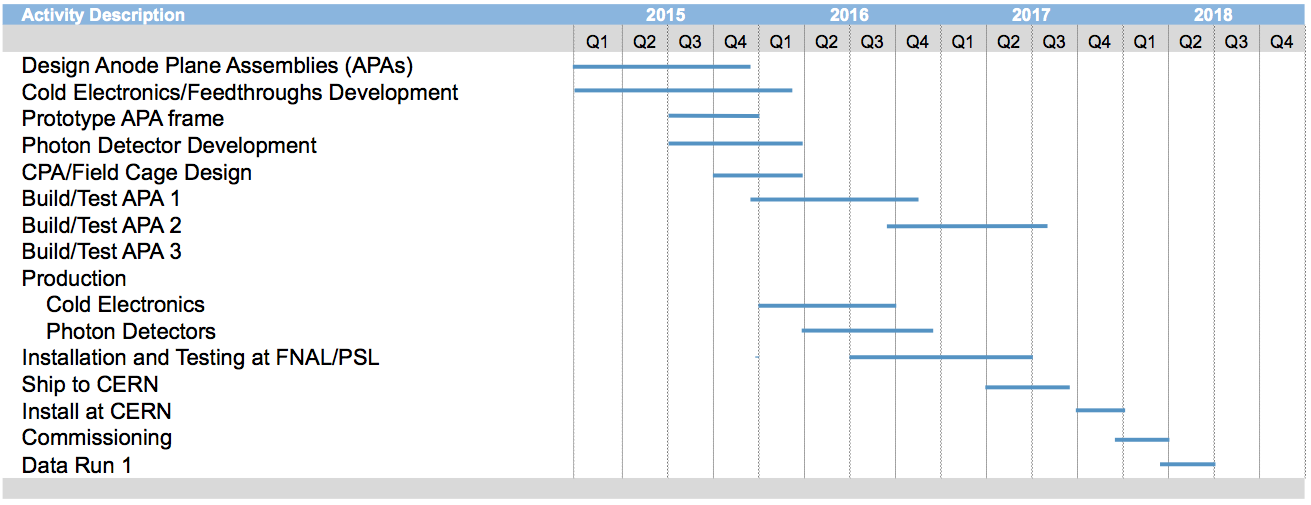
\includegraphics[scale=0.34]{figures/150219_schedule_3APAmod.png}
  \caption{Rolled up version of a draft schedule for manufacturing, installing and commissioning the CERN prototype detector. A 2 - 3 months data taking period is included in the schedule. }
  \label{fig:schedule}
\end{figure}


\subsection{Organization}

\begin{itemize}

\item working group structure and distributions of tasks/responsibilities

\end{itemize}



\subsection{Division of Responsibilities}

\subsubsection{Shared responsibilities}

The engineering design of the cryostat and the cryogenics system is considered to be a shared responsibility between ELBNF and CERN.


\subsubsection{ELBNF responsibilities}

The following detector components are expected to be covered by ELBNF project:
\begin{enumerate}
\item XX APAs
\item CPA
\item field cage
\item cold electronics
\item DAQ hardware and software
\item ...
\end{enumerate}



\subsubsection{CERN responsibilities}

\paragraph{The beam line} design, setup of the beam line and beam monitoring instrumentation are expected to be provided by CERN.

\paragraph{The cryostat and cryogenics system} are expected to be organized and paid for by the CERN nu-platform.
The scope of the EHN1 cryostat subsystem includes the design, procurement, fabrication, testing, delivery and oversight of a cryostat to contain the liquid argon and the TPC.\\
% moved here from chap 4 (by Anne)


The following items (incomplete list !) require further discussion. The responsibilities should be clearly spelled out.

\begin{itemize}

\item plans for data analysis and publications

\item describe overlap/commonalities with WA105 data analysis

\end{itemize}

